\chapter{[En curso] Estado del arte}
\label{chapter:estado_arte}

\chapquote{Solo sé que no se nada.}{Sócrates}


En este capítulo se introduce una revisión del estado del arte y del estado de la cuestión en lo que respecta al marco teórico del proyecto que se propone en este \gls{tfm}, así como una descripción sobre los sistemas que existen en el mercado o que han sido reportados en la literatura, los cuales presentan aspectos comunes con la solución propuesta.

\section{Análisis de la situación actual}

    En esta sección, se pone en valor y/o contraste la información introducida en las secciones anteriores, de tal forma que pueda realizarse un análisis del entorno en el que se desarrolla este proyecto, así como también se pueda poner de manifiesto la relevancia y la idoneidad del desarrollo propuesto. 
    
    \subsection{Monitorización mediante dispositivos biométricos}

        Durante los últimos años se han realizado numerosos experimentos en el ámbito científico con el objetivo de encontrar medidas biométricas que puedan servir de indicadores de algunos de los trastornos de salud mental con medidas biométricas, o bien patrones de comportamiento que también puedan servir de predictor.

        En un estudio comparativo del año 2021 \cite{hickey_smart_2021}, los investigadores realizaron una revisión de los 21 artículos publicados para tratar de identificar las medidas biométricas que permitan identificar depresión, ansiedad y estrés.

        Según este estudio, la \gls{vfc} es una medida muy utilizada para detectar estrés y ansiedad, mejorando su efectividad si se utiliza junto con \glspl{eeg}. Por otra parte, la \gls{eda} se vislumbra como otro buen indicador para el estrés, con la desventaja de su falta de fiabilidad. En cuanto a la depresión, se determinó un uso sistemático de los \glspl{eeg}, pero con dispositivos que no se encuentran a la venta en los mercados.

        En este área de trabajo se puede encontrar al estudio \textit{WESAD} \cite{schmidt_introducing_2018}, del año 2018. En este artículo fue construido un \gls{dataset} para la detección de estrés con datos de 15 voluntarios, mediante un dispositivo colocado en el pecho y otro en la muñeca. El primero de ellos se encargó de recoger datos de \glspl{ecg}, respiración y de movimiento (mediante acelerómetros), mientras que el segundo de ellos recogía datos de temperatura corporal, \gls{eda}, \gls{bvp} y nuevamente de movimiento mediante acelerómetros.

        Con estos datos se planteó un problema de clasificación binaria (estrés o ausencia del mismo) mediante diversos algoritmos (árboles de decisión, \textit{random forest}, k-vecinos más cercanos o \textit{KNN}), obteniéndose precisiones entre el 69\% y el 86\% si se utilizaban los datos del dispositivo de pecho y entre el 67\% y el 88\% para los correspondientes a la muñeca. Si el lector lo desea, puede consultar en \cite{schmidt_introducing_2018} las tablas del estudio donde se detalla la precisión por cada algoritmo y dato utilizado.

        En una línea similar el artículo \textit{PASS} \cite{parent_pass_2020} del año 2020 también plantea la construcción de un \gls{dataset} para la detección de estrés con datos de 48 participantes. La principal diferencia con el estudio anterior es el establecimiento de un entorno controlados para provocar cambios en los niveles de estrés a través de videojuegos; mientras que los datos recolectados son fundamentalmente los mismos: \glspl{ecg}, \gls{eda}, respiración, temperatura corporal y \glspl{eeg}.

        No obstante, los estudios anteriores construyeron \glspl{dataset} en condiciones de laboratorio, utilizando \glspl{invasiva} para la monitorización de las constantes de los voluntarios. En contraposición a estas mediciones, existen otros estudios que apuestan por un enfoque basados en \glspl{no-invasiva}, mediante \glspl{wearable} o con los propios teléfonos, siendo procedimientos más cercanos a los usuarios en su día a día. En este ámbito se puede encontrar los proyectos \textit{DemonicSalmon} \cite{boukhechba_demonicsalmon_2018} y \textit{StudentLife} \cite{rui_studentlife_2014}.

        \textit{DemonicSalmon} es un proyecto realizado en 2018, en el cual se monitorizó la salud mental mediante \glspl{smartphone}
        
        
        de 2018 de 72 universitarios entre 18 y 23 años. Datos no wearables: movilidad (que mejor la de la pulsera), actividad (aqui igual), patrones de comunicación. 
    
        
        Student life es el mitico de 2014, el de las 10 semanas con cuestionarios. Aqui usaban datos como micro, sensor de luz, gps, bluetooth y acelerometro para determinar actividad, conversacion,sueño y localizacion. 
        
        Sus cuestionarios de contraste con PSS, PHQ9 y UCLA pero solo ANTES y DESPUES de acabar el estudio, no diarios. Tirar con las correlaciones desde aqui.
    
    \subsection{Cuidado del bienestar emocional mediante aplicaciones móviles}

        La creciente digitalización de la sociedad impulsada por las aplicaciones móviles también se ha reflejado en el campo de la salud mental en los últimos años, con una gran variedad de iniciativas por parte de numerosos actores.

        Se puede considerar en primer lugar los esfuerzos \textit{oficiales} de Google y Apple para añadir nuevas funcionalidades a sus sistemas operativos, Android e iOS, respectivamente. En el caso de Google se trata de un componente nuevo \textit{Bienestar Digital} \cite{android_bienestar_nodate}, mientras que Apple decidió ampliar la funcionalidad de su aplicación \textit{Salud} \cite{noauthor_apple_2023}.
        
        La herramienta \textit{Bienestar Digital}, incluida por defecto en las nuevas versiones de Android, permite, entre otras funciones, establecer un modo descanso en el que no se reciben notificaciones; otro modo denominado \textit{sin distracciones} que pone temporalmente en pausa aplicaciones escogidas por el usuario, visualizar mediante \glspl{widget} y paneles estadísticas relacionadas con el uso de cada aplicación o la posibilidad de limitar el tiempo de uso de ciertas aplicaciones. En la Figura \ref{fig:estado_arte:bienestar_digital} se pueden ver ejemplos tomados desde el móvil del autor.

        \begin{figure}[h]
            \begin{subfigure}[t]{0.48\textwidth}
                \includegraphics[width=1\linewidth]{figures/Estadísticas uso.jpg}
            \end{subfigure}
            \hfill
            \begin{subfigure}[t]{0.49\textwidth}
                \includegraphics[width=1\linewidth]{figures/Limitador de aplicación.jpg}
            \end{subfigure}
            \caption{Ejemplos de las funciones de \textit{Bienestar Digital}}
            \label{fig:estado_arte:bienestar_digital}
        \end{figure}

        Por otra parte, en la versión 17 de iOS, fueron incorporadas a la aplicación \textit{Salud} características para que los usuarios reflexionaran sobre su estado de bienestar emocional, elementos de evaluación de ansiedad y depresión usados en los centros sanitarios, o estadísticas relacionadas con la salud visual. Nuevamente, se presentan algunos ejemplos en la Figura \ref{fig:estado_arte:ios_salud}.

        \begin{figure}[h]
            \begin{subfigure}[t]{0.49\textwidth}
                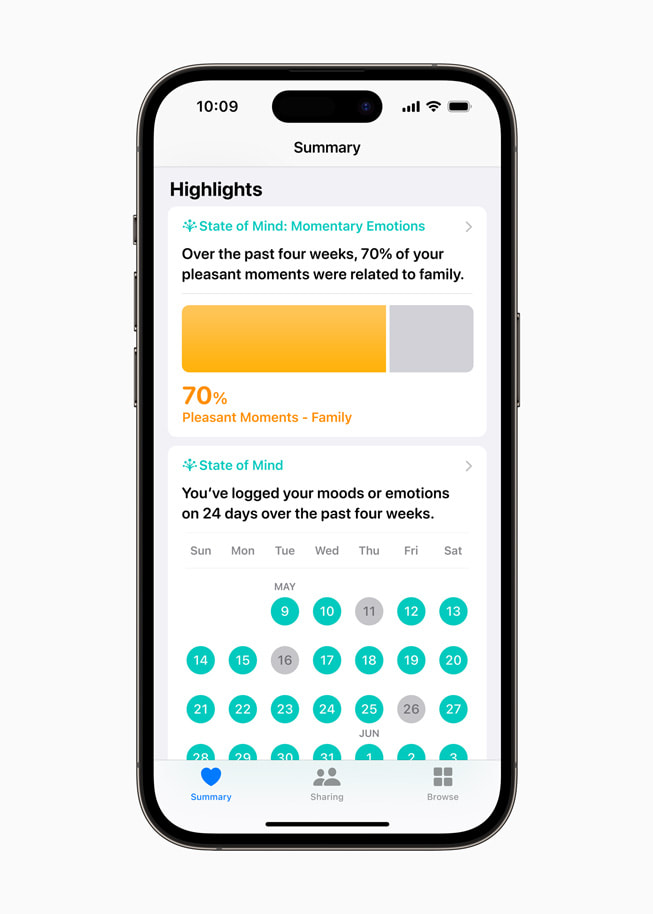
\includegraphics[width=1\linewidth]{figures/ios seguimiento bienestar emocional.jpg}
            \end{subfigure}
            \hfill
            \begin{subfigure}[t]{0.49\textwidth}
                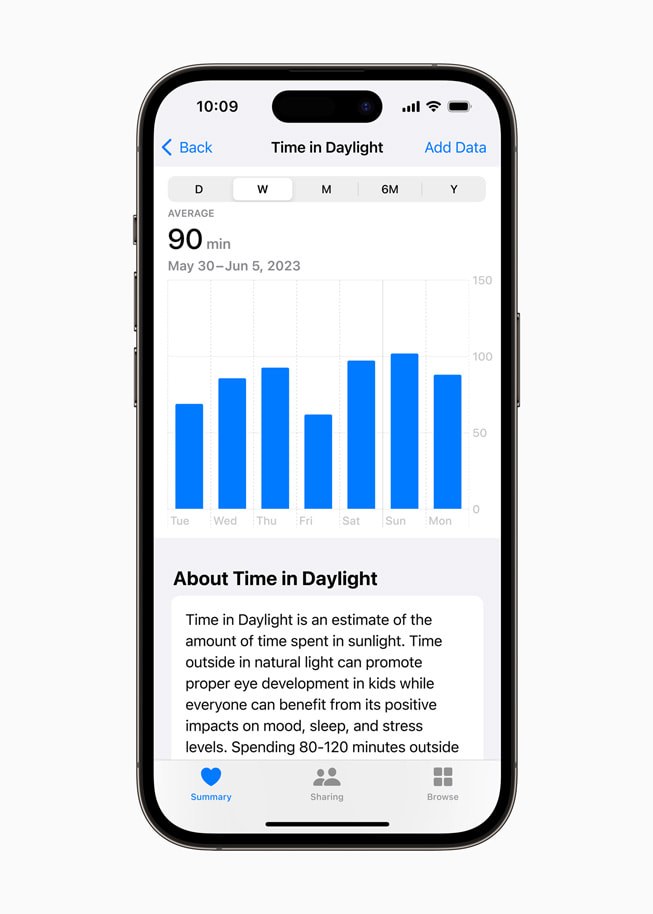
\includegraphics[width=1\linewidth]{figures/ios salud visual.jpg}
            \end{subfigure}
            \caption[Ejemplos de las funciones de bienestar de la aplicación \textit{Salud} de iOS]{Ejemplos de las funciones de bienestar de la aplicación \textit{Salud} de iOS, extraídos de \cite{noauthor_apple_2023}}
            \label{fig:estado_arte:ios_salud}
        \end{figure}

        En cuanto a las aplicaciones específicas desarrolladas por terceros, se trata de un mercado con gran proyección. El uso de estas aplicaciones creció, entre 2019 y 2021, un 54,6\% \cite{bejerano_lado_2023}, a la vez que el mercado global de estas apps se estimó en un valor aproximado de 6.200 millones de dólares en 2023; proyectándose un crecimiento incremento anual del 15,8\% hasta en 2030 según un análisis de \textit{Grand View Research} \cite{grand_view_research_mental_nodate}.
        
        Dentro de estas aplicaciones se pueden hallar varios enfoques. Por una parte existen plataformas como \textit{BetterHelp} o \textit{Talkspace}, las cuales hacen de intermediarios de usuarios con terapeutas, digitalizando el acceso al tratamiento. Otras como \textit{Happify} no recurren a profesionales y exploran el ámbito de la gamificación, incluyendo actividades y juegos para mejorar el estado de ánimo del usuario y que este tome un rol más activo. 
        
        Por otra parte, el planteamiento que se observa más común sea el de aplicaciones como \textit{Calm}, \textit{Yana} o \textit{Headspace}, las cuales se caracterizan por presentar meditaciones, música o ejercicios al usuario para reducir sus niveles, generalmente, de estrés \cite{modglin_5_2023} \cite{pepinosa_cinco_2023}. Para el acceso al contenido normalmente el usuario debe suscribirse, bien mensualmente o anualmente. 

        Estas aplicaciones presentan la ventaja de poder ser utilizadas en cualquier momento, a la vez que su precio suele ser notablemente inferior al coste de un tratamiento con un especialista. Suscripciones anuales como la de \textit{Calm} cuestan en torno a 65 euros anuales \cite{modglin_5_2023}, mientras que el coste de una consulta de una hora con un psicólogo asciende de media a 52 euros \cite{garcia_santos_boom_2023}. No obstante, el precio de una consulta no muestra el trabajo previo que realiza el profesional para preparar la sesión, ni tampoco muestra la diferencia en la atención al paciente.

        Sin embargo, las aplicaciones tienen una serie de desventajas claras. En primer lugar, para garantizar el rigor científico del contenido ofrecido se necesita que en su desarrollo trabajen profesionales especializados en salud mental, hecho que no suele reflejarse en la información de dichas aplicaciones. Asimismo, casos como el de \textit{Headspace}, una aplicación con más de 60 millones de usuarios, que fue creada por un \textit{``un monje budista tibetano y titulado en Artes Circenses en el Conservatorio de Danza y Teatro de Londres''} \cite{garcia_santos_boom_2023}, siembran ciertas dudas de su rigurosidad científica.
        
        En esta línea de trabajo se han realizado algunos trabajos científicos, debido a la popularidad de estas aplicaciones y su influencia en la salud mental en la sociedad. Según un análisis realizado en 2019 a 293 aplicaciones \cite{marshall_digital_2019}, solo el 3,41\% de las mismas presentaban pruebas científicas de su eficacia. \textit{``De estas 10 aplicaciones, sólo en tres casos la investigación era independiente; es decir, había sido realizada por una institución que no participaba en el desarrollo de la app''} \cite{garcia_santos_boom_2023}.

        Por otra parte, existen fundadas preocupaciones sobre la privacidad de dichas aplicaciones. Según un análisis de la Fundación Mozilla a 37 aplicaciones \cite{mozilla_foundation_privacidad_nodate}, a fecha de junio de 2024 22 de ellas fueron marcadas con la etiqueta \textit{privacidad no incluida}. Asimismo, se han reportado faltas de consentimiento para tratar datos confidenciales, ausencia de transparencia en los procesos o incluso, transcripciones de los chats entre los terapeutas y los usuarios. En el caso de \textit{Talkspace}, según dos ex-empleados \textit{``los científicos de datos de Talkspace compartían frases de estas transcripciones con el equipo de marketing para personalizar la publicidad de los usuarios''} \cite{bejerano_lado_2023}.
        
        En general, actualmente se pueden observar numerosas objeciones a estas aplicaciones tanto sobre su calidad como a la privacidad de los datos tratados, más teniendo en cuenta el impacto que pueden tener sobre la salud de las personas.

\section{Contribución de la solución propuesta}
    Usamos datos de wearables compatibles con varios fabricantes.
        health connect? Ya lo hablas en el contexto
    Cuestionarios diarios además de los de 12 semanas, tanto mañana y noche.